
% Default to the notebook output style

    


% Inherit from the specified cell style.




    
\documentclass[11pt,french]{article}

    
    \usepackage{babel}
    \usepackage[T1]{fontenc}
    % Nicer default font (+ math font) than Computer Modern for most use cases
    \usepackage{mathpazo}

    % Basic figure setup, for now with no caption control since it's done
    % automatically by Pandoc (which extracts ![](path) syntax from Markdown).
    \usepackage{graphicx}
    % We will generate all images so they have a width \maxwidth. This means
    % that they will get their normal width if they fit onto the page, but
    % are scaled down if they would overflow the margins.
    \makeatletter
    \def\maxwidth{\ifdim\Gin@nat@width>\linewidth\linewidth
    \else\Gin@nat@width\fi}
    \makeatother
    \let\Oldincludegraphics\includegraphics
    % Set max figure width to be 80% of text width, for now hardcoded.
    \renewcommand{\includegraphics}[1]{\Oldincludegraphics[width=.8\maxwidth]{#1}}
    % Ensure that by default, figures have no caption (until we provide a
    % proper Figure object with a Caption API and a way to capture that
    % in the conversion process - todo).
    \usepackage{caption}
    \DeclareCaptionLabelFormat{nolabel}{}
    \captionsetup{labelformat=nolabel}

    \usepackage{adjustbox} % Used to constrain images to a maximum size 
    \usepackage{xcolor} % Allow colors to be defined
    \usepackage{enumerate} % Needed for markdown enumerations to work
    \usepackage{geometry} % Used to adjust the document margins
    \usepackage{amsmath} % Equations
    \usepackage{amssymb} % Equations
    \usepackage{textcomp} % defines textquotesingle
    % Hack from http://tex.stackexchange.com/a/47451/13684:
    \AtBeginDocument{%
        \def\PYZsq{\textquotesingle}% Upright quotes in Pygmentized code
    }
    \usepackage{upquote} % Upright quotes for verbatim code
    \usepackage{eurosym} % defines \euro
    \usepackage[mathletters]{ucs} % Extended unicode (utf-8) support
    \usepackage[utf8x]{inputenc} % Allow utf-8 characters in the tex document
    \usepackage{fancyvrb} % verbatim replacement that allows latex
    \usepackage{grffile} % extends the file name processing of package graphics 
                         % to support a larger range 
    % The hyperref package gives us a pdf with properly built
    % internal navigation ('pdf bookmarks' for the table of contents,
    % internal cross-reference links, web links for URLs, etc.)
    \usepackage{hyperref}
    \usepackage{longtable} % longtable support required by pandoc >1.10
    \usepackage{booktabs}  % table support for pandoc > 1.12.2
    \usepackage[inline]{enumitem} % IRkernel/repr support (it uses the enumerate* environment)
    \usepackage[normalem]{ulem} % ulem is needed to support strikethroughs (\sout)
                                % normalem makes italics be italics, not underlines
    \usepackage{mathrsfs}
    

    
    
    % Colors for the hyperref package
    \definecolor{urlcolor}{rgb}{0,.145,.698}
    \definecolor{linkcolor}{rgb}{.71,0.21,0.01}
    \definecolor{citecolor}{rgb}{.12,.54,.11}

    % ANSI colors
    \definecolor{ansi-black}{HTML}{3E424D}
    \definecolor{ansi-black-intense}{HTML}{282C36}
    \definecolor{ansi-red}{HTML}{E75C58}
    \definecolor{ansi-red-intense}{HTML}{B22B31}
    \definecolor{ansi-green}{HTML}{00A250}
    \definecolor{ansi-green-intense}{HTML}{007427}
    \definecolor{ansi-yellow}{HTML}{DDB62B}
    \definecolor{ansi-yellow-intense}{HTML}{B27D12}
    \definecolor{ansi-blue}{HTML}{208FFB}
    \definecolor{ansi-blue-intense}{HTML}{0065CA}
    \definecolor{ansi-magenta}{HTML}{D160C4}
    \definecolor{ansi-magenta-intense}{HTML}{A03196}
    \definecolor{ansi-cyan}{HTML}{60C6C8}
    \definecolor{ansi-cyan-intense}{HTML}{258F8F}
    \definecolor{ansi-white}{HTML}{C5C1B4}
    \definecolor{ansi-white-intense}{HTML}{A1A6B2}
    \definecolor{ansi-default-inverse-fg}{HTML}{FFFFFF}
    \definecolor{ansi-default-inverse-bg}{HTML}{000000}

    % commands and environments needed by pandoc snippets
    % extracted from the output of `pandoc -s`
    \providecommand{\tightlist}{%
      \setlength{\itemsep}{0pt}\setlength{\parskip}{0pt}}
    \DefineVerbatimEnvironment{Highlighting}{Verbatim}{commandchars=\\\{\}}
    % Add ',fontsize=\small' for more characters per line
    \newenvironment{Shaded}{}{}
    \newcommand{\KeywordTok}[1]{\textcolor[rgb]{0.00,0.44,0.13}{\textbf{{#1}}}}
    \newcommand{\DataTypeTok}[1]{\textcolor[rgb]{0.56,0.13,0.00}{{#1}}}
    \newcommand{\DecValTok}[1]{\textcolor[rgb]{0.25,0.63,0.44}{{#1}}}
    \newcommand{\BaseNTok}[1]{\textcolor[rgb]{0.25,0.63,0.44}{{#1}}}
    \newcommand{\FloatTok}[1]{\textcolor[rgb]{0.25,0.63,0.44}{{#1}}}
    \newcommand{\CharTok}[1]{\textcolor[rgb]{0.25,0.44,0.63}{{#1}}}
    \newcommand{\StringTok}[1]{\textcolor[rgb]{0.25,0.44,0.63}{{#1}}}
    \newcommand{\CommentTok}[1]{\textcolor[rgb]{0.38,0.63,0.69}{\textit{{#1}}}}
    \newcommand{\OtherTok}[1]{\textcolor[rgb]{0.00,0.44,0.13}{{#1}}}
    \newcommand{\AlertTok}[1]{\textcolor[rgb]{1.00,0.00,0.00}{\textbf{{#1}}}}
    \newcommand{\FunctionTok}[1]{\textcolor[rgb]{0.02,0.16,0.49}{{#1}}}
    \newcommand{\RegionMarkerTok}[1]{{#1}}
    \newcommand{\ErrorTok}[1]{\textcolor[rgb]{1.00,0.00,0.00}{\textbf{{#1}}}}
    \newcommand{\NormalTok}[1]{{#1}}
    
    % Additional commands for more recent versions of Pandoc
    \newcommand{\ConstantTok}[1]{\textcolor[rgb]{0.53,0.00,0.00}{{#1}}}
    \newcommand{\SpecialCharTok}[1]{\textcolor[rgb]{0.25,0.44,0.63}{{#1}}}
    \newcommand{\VerbatimStringTok}[1]{\textcolor[rgb]{0.25,0.44,0.63}{{#1}}}
    \newcommand{\SpecialStringTok}[1]{\textcolor[rgb]{0.73,0.40,0.53}{{#1}}}
    \newcommand{\ImportTok}[1]{{#1}}
    \newcommand{\DocumentationTok}[1]{\textcolor[rgb]{0.73,0.13,0.13}{\textit{{#1}}}}
    \newcommand{\AnnotationTok}[1]{\textcolor[rgb]{0.38,0.63,0.69}{\textbf{\textit{{#1}}}}}
    \newcommand{\CommentVarTok}[1]{\textcolor[rgb]{0.38,0.63,0.69}{\textbf{\textit{{#1}}}}}
    \newcommand{\VariableTok}[1]{\textcolor[rgb]{0.10,0.09,0.49}{{#1}}}
    \newcommand{\ControlFlowTok}[1]{\textcolor[rgb]{0.00,0.44,0.13}{\textbf{{#1}}}}
    \newcommand{\OperatorTok}[1]{\textcolor[rgb]{0.40,0.40,0.40}{{#1}}}
    \newcommand{\BuiltInTok}[1]{{#1}}
    \newcommand{\ExtensionTok}[1]{{#1}}
    \newcommand{\PreprocessorTok}[1]{\textcolor[rgb]{0.74,0.48,0.00}{{#1}}}
    \newcommand{\AttributeTok}[1]{\textcolor[rgb]{0.49,0.56,0.16}{{#1}}}
    \newcommand{\InformationTok}[1]{\textcolor[rgb]{0.38,0.63,0.69}{\textbf{\textit{{#1}}}}}
    \newcommand{\WarningTok}[1]{\textcolor[rgb]{0.38,0.63,0.69}{\textbf{\textit{{#1}}}}}
    
    
    % Define a nice break command that doesn't care if a line doesn't already
    % exist.
    \def\br{\hspace*{\fill} \\* }
    % Math Jax compatibility definitions
    \def\gt{>}
    \def\lt{<}
    \let\Oldtex\TeX
    \let\Oldlatex\LaTeX
    \renewcommand{\TeX}{\textrm{\Oldtex}}
    \renewcommand{\LaTeX}{\textrm{\Oldlatex}}
    % Document parameters
    % Document title
    \title{Architecture de Von Neumann et ses alternatives. Description et état des lieux}
    
    
    
    
    

    % Pygments definitions
    
\makeatletter
\def\PY@reset{\let\PY@it=\relax \let\PY@bf=\relax%
    \let\PY@ul=\relax \let\PY@tc=\relax%
    \let\PY@bc=\relax \let\PY@ff=\relax}
\def\PY@tok#1{\csname PY@tok@#1\endcsname}
\def\PY@toks#1+{\ifx\relax#1\empty\else%
    \PY@tok{#1}\expandafter\PY@toks\fi}
\def\PY@do#1{\PY@bc{\PY@tc{\PY@ul{%
    \PY@it{\PY@bf{\PY@ff{#1}}}}}}}
\def\PY#1#2{\PY@reset\PY@toks#1+\relax+\PY@do{#2}}

\expandafter\def\csname PY@tok@w\endcsname{\def\PY@tc##1{\textcolor[rgb]{0.73,0.73,0.73}{##1}}}
\expandafter\def\csname PY@tok@c\endcsname{\let\PY@it=\textit\def\PY@tc##1{\textcolor[rgb]{0.25,0.50,0.50}{##1}}}
\expandafter\def\csname PY@tok@cp\endcsname{\def\PY@tc##1{\textcolor[rgb]{0.74,0.48,0.00}{##1}}}
\expandafter\def\csname PY@tok@k\endcsname{\let\PY@bf=\textbf\def\PY@tc##1{\textcolor[rgb]{0.00,0.50,0.00}{##1}}}
\expandafter\def\csname PY@tok@kp\endcsname{\def\PY@tc##1{\textcolor[rgb]{0.00,0.50,0.00}{##1}}}
\expandafter\def\csname PY@tok@kt\endcsname{\def\PY@tc##1{\textcolor[rgb]{0.69,0.00,0.25}{##1}}}
\expandafter\def\csname PY@tok@o\endcsname{\def\PY@tc##1{\textcolor[rgb]{0.40,0.40,0.40}{##1}}}
\expandafter\def\csname PY@tok@ow\endcsname{\let\PY@bf=\textbf\def\PY@tc##1{\textcolor[rgb]{0.67,0.13,1.00}{##1}}}
\expandafter\def\csname PY@tok@nb\endcsname{\def\PY@tc##1{\textcolor[rgb]{0.00,0.50,0.00}{##1}}}
\expandafter\def\csname PY@tok@nf\endcsname{\def\PY@tc##1{\textcolor[rgb]{0.00,0.00,1.00}{##1}}}
\expandafter\def\csname PY@tok@nc\endcsname{\let\PY@bf=\textbf\def\PY@tc##1{\textcolor[rgb]{0.00,0.00,1.00}{##1}}}
\expandafter\def\csname PY@tok@nn\endcsname{\let\PY@bf=\textbf\def\PY@tc##1{\textcolor[rgb]{0.00,0.00,1.00}{##1}}}
\expandafter\def\csname PY@tok@ne\endcsname{\let\PY@bf=\textbf\def\PY@tc##1{\textcolor[rgb]{0.82,0.25,0.23}{##1}}}
\expandafter\def\csname PY@tok@nv\endcsname{\def\PY@tc##1{\textcolor[rgb]{0.10,0.09,0.49}{##1}}}
\expandafter\def\csname PY@tok@no\endcsname{\def\PY@tc##1{\textcolor[rgb]{0.53,0.00,0.00}{##1}}}
\expandafter\def\csname PY@tok@nl\endcsname{\def\PY@tc##1{\textcolor[rgb]{0.63,0.63,0.00}{##1}}}
\expandafter\def\csname PY@tok@ni\endcsname{\let\PY@bf=\textbf\def\PY@tc##1{\textcolor[rgb]{0.60,0.60,0.60}{##1}}}
\expandafter\def\csname PY@tok@na\endcsname{\def\PY@tc##1{\textcolor[rgb]{0.49,0.56,0.16}{##1}}}
\expandafter\def\csname PY@tok@nt\endcsname{\let\PY@bf=\textbf\def\PY@tc##1{\textcolor[rgb]{0.00,0.50,0.00}{##1}}}
\expandafter\def\csname PY@tok@nd\endcsname{\def\PY@tc##1{\textcolor[rgb]{0.67,0.13,1.00}{##1}}}
\expandafter\def\csname PY@tok@s\endcsname{\def\PY@tc##1{\textcolor[rgb]{0.73,0.13,0.13}{##1}}}
\expandafter\def\csname PY@tok@sd\endcsname{\let\PY@it=\textit\def\PY@tc##1{\textcolor[rgb]{0.73,0.13,0.13}{##1}}}
\expandafter\def\csname PY@tok@si\endcsname{\let\PY@bf=\textbf\def\PY@tc##1{\textcolor[rgb]{0.73,0.40,0.53}{##1}}}
\expandafter\def\csname PY@tok@se\endcsname{\let\PY@bf=\textbf\def\PY@tc##1{\textcolor[rgb]{0.73,0.40,0.13}{##1}}}
\expandafter\def\csname PY@tok@sr\endcsname{\def\PY@tc##1{\textcolor[rgb]{0.73,0.40,0.53}{##1}}}
\expandafter\def\csname PY@tok@ss\endcsname{\def\PY@tc##1{\textcolor[rgb]{0.10,0.09,0.49}{##1}}}
\expandafter\def\csname PY@tok@sx\endcsname{\def\PY@tc##1{\textcolor[rgb]{0.00,0.50,0.00}{##1}}}
\expandafter\def\csname PY@tok@m\endcsname{\def\PY@tc##1{\textcolor[rgb]{0.40,0.40,0.40}{##1}}}
\expandafter\def\csname PY@tok@gh\endcsname{\let\PY@bf=\textbf\def\PY@tc##1{\textcolor[rgb]{0.00,0.00,0.50}{##1}}}
\expandafter\def\csname PY@tok@gu\endcsname{\let\PY@bf=\textbf\def\PY@tc##1{\textcolor[rgb]{0.50,0.00,0.50}{##1}}}
\expandafter\def\csname PY@tok@gd\endcsname{\def\PY@tc##1{\textcolor[rgb]{0.63,0.00,0.00}{##1}}}
\expandafter\def\csname PY@tok@gi\endcsname{\def\PY@tc##1{\textcolor[rgb]{0.00,0.63,0.00}{##1}}}
\expandafter\def\csname PY@tok@gr\endcsname{\def\PY@tc##1{\textcolor[rgb]{1.00,0.00,0.00}{##1}}}
\expandafter\def\csname PY@tok@ge\endcsname{\let\PY@it=\textit}
\expandafter\def\csname PY@tok@gs\endcsname{\let\PY@bf=\textbf}
\expandafter\def\csname PY@tok@gp\endcsname{\let\PY@bf=\textbf\def\PY@tc##1{\textcolor[rgb]{0.00,0.00,0.50}{##1}}}
\expandafter\def\csname PY@tok@go\endcsname{\def\PY@tc##1{\textcolor[rgb]{0.53,0.53,0.53}{##1}}}
\expandafter\def\csname PY@tok@gt\endcsname{\def\PY@tc##1{\textcolor[rgb]{0.00,0.27,0.87}{##1}}}
\expandafter\def\csname PY@tok@err\endcsname{\def\PY@bc##1{\setlength{\fboxsep}{0pt}\fcolorbox[rgb]{1.00,0.00,0.00}{1,1,1}{\strut ##1}}}
\expandafter\def\csname PY@tok@kc\endcsname{\let\PY@bf=\textbf\def\PY@tc##1{\textcolor[rgb]{0.00,0.50,0.00}{##1}}}
\expandafter\def\csname PY@tok@kd\endcsname{\let\PY@bf=\textbf\def\PY@tc##1{\textcolor[rgb]{0.00,0.50,0.00}{##1}}}
\expandafter\def\csname PY@tok@kn\endcsname{\let\PY@bf=\textbf\def\PY@tc##1{\textcolor[rgb]{0.00,0.50,0.00}{##1}}}
\expandafter\def\csname PY@tok@kr\endcsname{\let\PY@bf=\textbf\def\PY@tc##1{\textcolor[rgb]{0.00,0.50,0.00}{##1}}}
\expandafter\def\csname PY@tok@bp\endcsname{\def\PY@tc##1{\textcolor[rgb]{0.00,0.50,0.00}{##1}}}
\expandafter\def\csname PY@tok@fm\endcsname{\def\PY@tc##1{\textcolor[rgb]{0.00,0.00,1.00}{##1}}}
\expandafter\def\csname PY@tok@vc\endcsname{\def\PY@tc##1{\textcolor[rgb]{0.10,0.09,0.49}{##1}}}
\expandafter\def\csname PY@tok@vg\endcsname{\def\PY@tc##1{\textcolor[rgb]{0.10,0.09,0.49}{##1}}}
\expandafter\def\csname PY@tok@vi\endcsname{\def\PY@tc##1{\textcolor[rgb]{0.10,0.09,0.49}{##1}}}
\expandafter\def\csname PY@tok@vm\endcsname{\def\PY@tc##1{\textcolor[rgb]{0.10,0.09,0.49}{##1}}}
\expandafter\def\csname PY@tok@sa\endcsname{\def\PY@tc##1{\textcolor[rgb]{0.73,0.13,0.13}{##1}}}
\expandafter\def\csname PY@tok@sb\endcsname{\def\PY@tc##1{\textcolor[rgb]{0.73,0.13,0.13}{##1}}}
\expandafter\def\csname PY@tok@sc\endcsname{\def\PY@tc##1{\textcolor[rgb]{0.73,0.13,0.13}{##1}}}
\expandafter\def\csname PY@tok@dl\endcsname{\def\PY@tc##1{\textcolor[rgb]{0.73,0.13,0.13}{##1}}}
\expandafter\def\csname PY@tok@s2\endcsname{\def\PY@tc##1{\textcolor[rgb]{0.73,0.13,0.13}{##1}}}
\expandafter\def\csname PY@tok@sh\endcsname{\def\PY@tc##1{\textcolor[rgb]{0.73,0.13,0.13}{##1}}}
\expandafter\def\csname PY@tok@s1\endcsname{\def\PY@tc##1{\textcolor[rgb]{0.73,0.13,0.13}{##1}}}
\expandafter\def\csname PY@tok@mb\endcsname{\def\PY@tc##1{\textcolor[rgb]{0.40,0.40,0.40}{##1}}}
\expandafter\def\csname PY@tok@mf\endcsname{\def\PY@tc##1{\textcolor[rgb]{0.40,0.40,0.40}{##1}}}
\expandafter\def\csname PY@tok@mh\endcsname{\def\PY@tc##1{\textcolor[rgb]{0.40,0.40,0.40}{##1}}}
\expandafter\def\csname PY@tok@mi\endcsname{\def\PY@tc##1{\textcolor[rgb]{0.40,0.40,0.40}{##1}}}
\expandafter\def\csname PY@tok@il\endcsname{\def\PY@tc##1{\textcolor[rgb]{0.40,0.40,0.40}{##1}}}
\expandafter\def\csname PY@tok@mo\endcsname{\def\PY@tc##1{\textcolor[rgb]{0.40,0.40,0.40}{##1}}}
\expandafter\def\csname PY@tok@ch\endcsname{\let\PY@it=\textit\def\PY@tc##1{\textcolor[rgb]{0.25,0.50,0.50}{##1}}}
\expandafter\def\csname PY@tok@cm\endcsname{\let\PY@it=\textit\def\PY@tc##1{\textcolor[rgb]{0.25,0.50,0.50}{##1}}}
\expandafter\def\csname PY@tok@cpf\endcsname{\let\PY@it=\textit\def\PY@tc##1{\textcolor[rgb]{0.25,0.50,0.50}{##1}}}
\expandafter\def\csname PY@tok@c1\endcsname{\let\PY@it=\textit\def\PY@tc##1{\textcolor[rgb]{0.25,0.50,0.50}{##1}}}
\expandafter\def\csname PY@tok@cs\endcsname{\let\PY@it=\textit\def\PY@tc##1{\textcolor[rgb]{0.25,0.50,0.50}{##1}}}

\def\PYZbs{\char`\\}
\def\PYZus{\char`\_}
\def\PYZob{\char`\{}
\def\PYZcb{\char`\}}
\def\PYZca{\char`\^}
\def\PYZam{\char`\&}
\def\PYZlt{\char`\<}
\def\PYZgt{\char`\>}
\def\PYZsh{\char`\#}
\def\PYZpc{\char`\%}
\def\PYZdl{\char`\$}
\def\PYZhy{\char`\-}
\def\PYZsq{\char`\'}
\def\PYZdq{\char`\"}
\def\PYZti{\char`\~}
% for compatibility with earlier versions
\def\PYZat{@}
\def\PYZlb{[}
\def\PYZrb{]}
\makeatother


    % Exact colors from NB
    \definecolor{incolor}{rgb}{0.0, 0.0, 0.5}
    \definecolor{outcolor}{rgb}{0.545, 0.0, 0.0}



    
    % Prevent overflowing lines due to hard-to-break entities
    \sloppy 
    % Setup hyperref package
    \hypersetup{
      breaklinks=true,  % so long urls are correctly broken across lines
      colorlinks=true,
      urlcolor=urlcolor,
      linkcolor=linkcolor,
      citecolor=citecolor,
      }
    % Slightly bigger margins than the latex defaults
    
    \geometry{verbose,tmargin=1in,bmargin=1in,lmargin=1in,rmargin=1in}
    
    
	\author{\textsc{Bruno Darid}}
    \begin{document}
    \renewcommand{\contentsname}{\textsc{Plan}}    
 	\maketitle
 	\tableofcontents
    
    

    
    \hypertarget{repuxe8res-historiques}{%
\section{Repères historiques}\label{repuxe8res-historiques}}

%Les années 40 furent riches en termes de développement des
%\href{https://fr.wikipedia.org/wiki/Histoire_des_ordinateurs}{premiers
%calculateurs programmables}. Cependant, les programmes étaient externes
%(sur \emph{cartes perforées}) avec tous les inconvénients que cela
%suppose (\emph{vitesse d'exécution notamment}).\\
%En 1945, un brillant mathématicien physicien,
%\href{https://fr.wikipedia.org/wiki/John_von_Neumann}{John von Neumann} (fig. \ref{fig:vonneumann})
%décrit dans un rapport la structure d'un nouveau calculateur: le
%\textbf{calculateur à programme enregistré}. Il dirigea sa construction
%jusqu'en 1952. 

\hypertarget{repuxe8res-historiques}{%
\section{Repères historiques}\label{repuxe8res-historiques}}
\begin{figure}[h]
	\begin{center}
		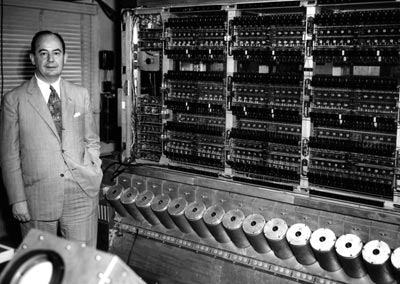
\includegraphics{../img/IAS_von_Neumann.jpg}
	\end{center}
	\caption{Fig. \ref{fig:vonneumann} -- John Von Neumann}
	\label{fig:vonneumann}
\end{figure}
	
    \hypertarget{moduxe8le-darchitecture-suxe9quentielle-dite-de-von-neumann}{%
\section{\texorpdfstring{Modèle d'architecture séquentielle (\emph{dite
de von
Neumann})}{Modèle d'architecture séquentielle (dite de von Neumann)}}\label{moduxe8le-darchitecture-suxe9quentielle-dite-de-von-neumann}}

Dans son rapport de 1945, John von Neumann énumère les principaux
organes de cette nouvelle machine:
\begin{itemize}
\item le processeur; 
\item la mémoire; 
\item les dispositifs d'entrée/sortie
\end{itemize}

L'idée fondamentale est de stocker les données \textbf{et} les
instructions des programmes en mémoire centrale.

\hypertarget{les-composants-essentiels}{%
\subsection{Les composants essentiels}\label{les-composants-essentiels}}

En juin 1945 dans la première version du rapport sur la conception de
\href{https://fr.wikipedia.org/wiki/Electronic_Discrete_Variable_Automatic_Computer}{l'EDVAC}
John von Neumann décrit un schéma d'architecture d'un calculateur
organisé autour des éléments suivants:
\begin{itemize}
\item une unité arithmétique et logique (\emph{UAL}); 
\item une unité de commande (\emph{Control Unit}); 
\item la mémoire; 
\item des unités d'entrées/sorties.
\end{itemize}
Ces éléments étant reliés entre eux par des bus.

\begin{figure}[h]
	\begin{center}
		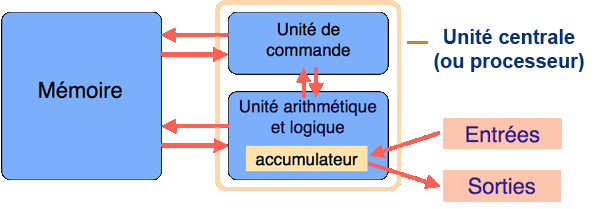
\includegraphics{../img/modele-originel2.png}
	\end{center}
	\caption{Fig. \ref{fig:modeloriginal} -- Modèle original}
	\label{fig:modeloriginal}
\end{figure}

L'UAL et l'unité de contrôle forment le \textbf{processeur}; on dit aussi \textbf{CPU} pour \textbf{C}entral
\textbf{P}rocessing \textbf{U}nit.

\hypertarget{uniteAL}{%
\subsection{L'unité arithmétique et logique}\label{uniteAL}}

 Elle est chargée d'effectuer le traitements des opérations   arithmétiques ou booléennes:
\begin{itemize}
\tightlist
\item addition, multiplication, soustraction, division
\item ET, OU et NON logiques;
\item décalages de bits dans des registres
\end{itemize}

L'UAL est entourée généralement de \textbf{registres de données}
(\textit{mémoires rapides}) et d'un \textbf{accumulateur} qui accueille les opérandes des
opérations ou le résultat.

\hypertarget{unitcontrol}{%
\subsection{L'unité de contrôle}\label{unitcontrol}}

  Elle est chargée de contrôler les échanges, gérer l'enchainement des
  instructions et les transferts entre les différents éléments.
\begin{figure}[h]
	\begin{center}  
  		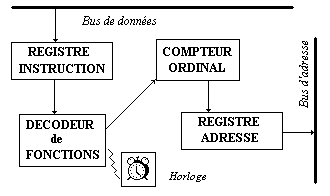
\includegraphics{../img/control_unit.png} 
	\end{center}
	\caption{Fig. \ref{fig:controlunit} -- Unité de contrôle}
	\label{fig:controlunit}
\end{figure}

On y trouve (\textit{entre autres}):

\begin{itemize}
\tightlist
\item
  un compteur ordinal ou \og Program Counter PC\fg  qui contient l'adresse
  de la prochaine instruction;
\item
  un registre d'instruction  ou \og Instruction Register IR  ou Current Instruction
  Register CIR\fg qui contient l'instruction lue;
\item
  un décodeur d'instruction;
\item
  un registre d'adresse ou \og Memory Address Register MAR\fg qui contient
  l'adresse mémoire de l'instruction à lire;
\item   une horloge.
\end{itemize}

\hypertarget{les-memoires}{%
\subsection{Les mémoires}\label{les-memoires}}
Le rôle des mémoires est d'enregistrer les programmes et les données pouvant être executées par le microprocesseur. On peut classer les mémoires en deux grandes catégories:
\begin{itemize}
    \item les mémoires de travail;
    \item les mémoires de stockage.
\end{itemize}
Les mémoires vives ou RAM (\textit{Random Access Memory}) permettent des opérations de lecture et d'écriture. Elles sont volatiles. Les mémoires accessibles uniquement en lecture sont connues sous le nom de ROM (\textit{Read Only Memory}).

Les mémoires de stockage (ou mémoire de masse) se présentent souvent sous la forme de disque.
Même si la fonction est la même (\textit{mémorisation de l'information}), toutes ces mémoires ont des caractéristiques différentes:

\begin{figure}[h]
	\begin{center}
		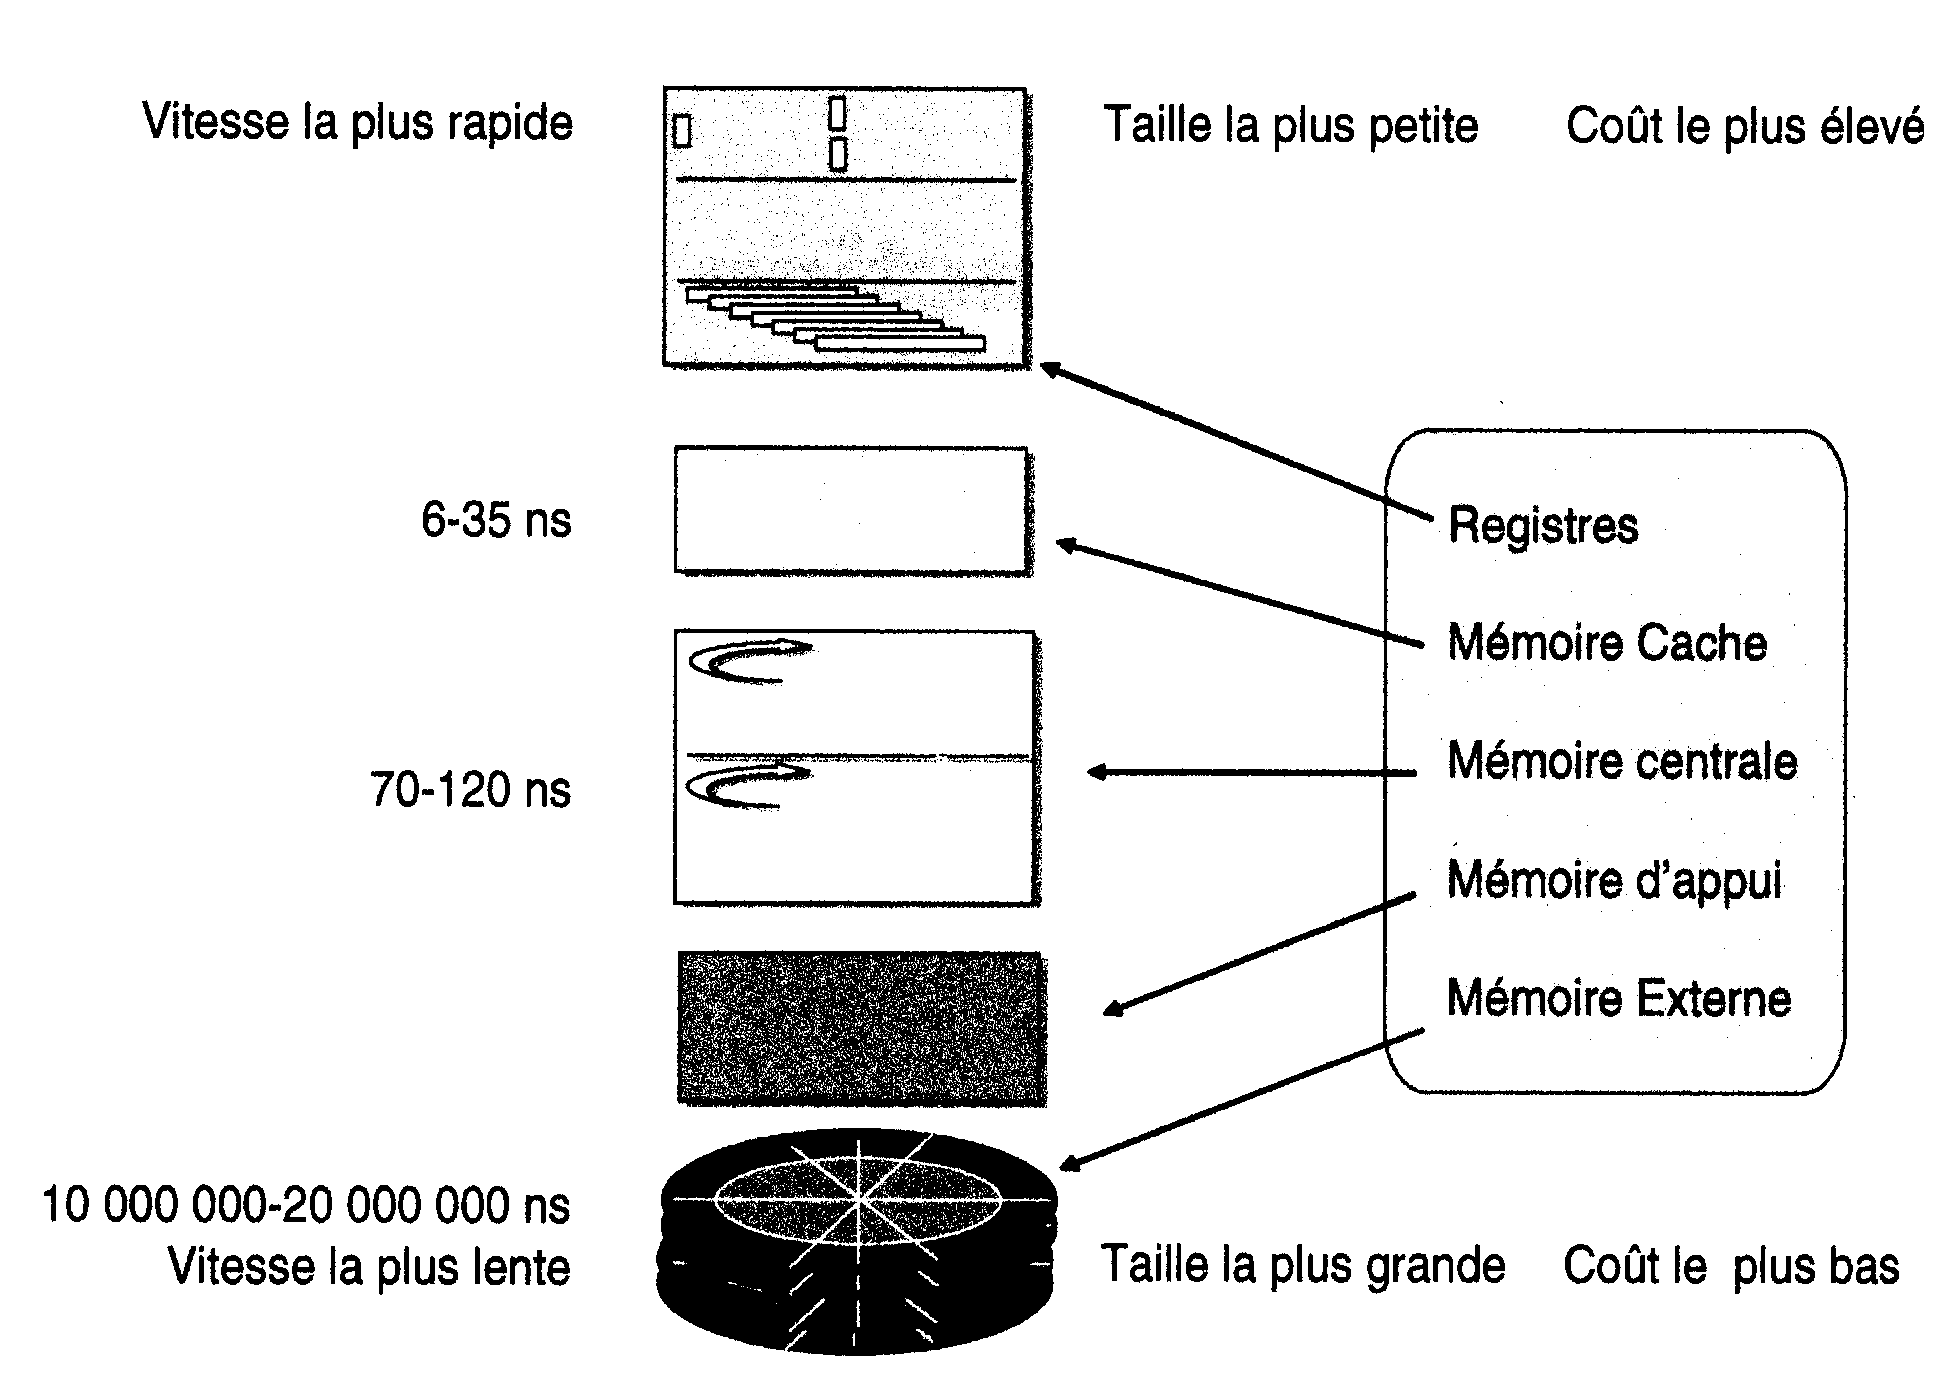
\includegraphics{../img/DiU001.png}
	\end{center}
	\caption{Fig. \ref{fig:memoires} -- Les mémoires}
	\label{fig:memoires}
\end{figure}

\hypertarget{les-bus}{%
\subsection{Les bus}\label{les-bus}}
  Les différentes unités sont interconnectées par des systèmes de
  câblage appelé bus. Autour du processeur on trouve:


\begin{itemize}
\tightlist
\item
  le bus d'adresse unidirectionnel;
\item
  le bus de données bidirectionnel;
\item
  le bus de contrôle bidirectionnel.
\end{itemize}

\emph{Remarque}: les ordinateurs récents possèdent d'autres types de
bus.

\hypertarget{les-instructions}{%
\subsection{Les instructions}\label{les-instructions}}

Une instruction désigne un ordre donné au processeur. Il s'agit d'une
chaine binaire de \(p\) bits composée de deux parties.
\begin{figure}[h]
	\begin{center}
		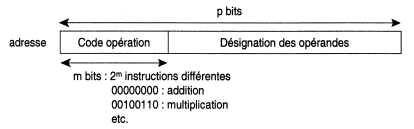
\includegraphics{../img/as_instruction.jpg} 
	\end{center}
	\caption{Fig. \ref{fig:les-instructions} -- Format d'une instruction}
	\label{fig:les-instructions}
\end{figure}

Pour s'affranchir des codes
binaires et des calculs d'adresse le programmeur utilise plutôt un
\textbf{langage d'assemblage} où les instructions binaires sont
remplacés par une chaine de caractères mnémoniques. Un programme appelé
\textbf{assembleur} réalisera ensuite le passage vers le code binaire.\par
Les intructions du langage machine peuvent être rangées dans six
catégories: calcul, transfert, entrées/sorties, saut, appel de sous
programme, instructions particulières (arrêt par exemple).\\
L'ensemble des codes opération reconnu par un processeur s'appelle son
\emph{jeu d'instructions}.\\ 

\textbf{Il n'est pas question dans ce cours de
détailler un quelconque jeu d'instructions, ni les subtilités de son
utilisation. Il s'agit plutôt de présenter quelques séquences simples}.\\

Dans les exemples qui suivront le jeu d'instructions minimaliste utilisé
(\textit{voisin de celui des processeurs
\href{https://fr.wikipedia.org/wiki/Architecture_ARM}{ARM}}) peut être
trouvé \href{http://www.peterhigginson.co.uk/AQA/info.html}{à cette
adresse}. Les commentaires sont précédés du caractère \texttt{;}. 

\hypertarget{exemple-1}{%
\subsubsection{Exemple commenté \no 1}\label{exemple-1}}
\begin{verbatim}
  MOV R0,#30;chargement du registre R0 avec la valeur 30
  MOV R1,#20
  ADD R2,R1,R0;additionne les contenus de R0 et R1 et place le contenu dans le registre R2
  STR R2,100;transfert le contenu de R2 à l'adresse 100
  HALT;arret des traitements
\end{verbatim}

\hypertarget{exemple-2}{%
\subsubsection{Exemple commenté \no2}\label{exemple-2}}
\begin{verbatim}
  0       MOV R0,#30
  1       MOV R1,#20
  2       MOV R3,#0
  3       ADD R2,R1,R0
  4       CMP R2,#0
  5 si:   BNE fin
  6       MOV R2,R3
  7 fin:  HALT
\end{verbatim}
Dans cet exemple, on introduit la possibilité d'introduire des
\emph{étiquettes} utiles pour réaliser des sauts. Elles évitent d'avoir à
calculer l'adresse de l'instruction en question (\emph{laissant ce
travail à l'assembleur}). La structure présentée ici est équivalente à
un test sans alternatives.

\hypertarget{e1c5-que-fait-cette-suxe9quence-dinstructions}{%
\subsubsection{E1C5 Que fait cette séquence
d'instructions?}\label{e1c5-que-fait-cette-suxe9quence-dinstructions}}
\begin{enumerate}
\item Expliquer ce réalise les instructions ci-dessous:
	\begin{verbatim}
	 MOV R0,#25
      STR R0,20
      MOV R1,#6
      STR R1,21
      ADD R0,R1,R0
      LSL R0,R0,#1
      STR R0,22
      HALT
	\end{verbatim}
\item Vérifier vos résultats avec le simulateur de
\href{http://www.peterhigginson.co.uk/AQA/}{Peter Higginson}.
\end{enumerate}

\hypertarget{e2c5-langage-dassemblage}{%
\subsubsection{E2C5 Langage
d'assemblage}\label{e2c5-langage-dassemblage}}

Écrire en langage d'assemblage les instructions correspondant aux
actions suivantes :
\begin{itemize}
\item[$\vartriangleright$] comparer la valeur du registre R4 avec la valeur 18 (décimale)
\item[$\vartriangleright$] si celle-ci est plus grande alors sauter à l'étiquette `etiqu1'
\item[$\vartriangleright$] charger la valeur 14 dans le registre R0; 
\item[$\vartriangleright$] arrêter les traitements 
\item[$\vartriangleright$] déclarer l'étiquette `etiqu1' 
\item[$\vartriangleright$] charger la valeur 18 dans le registre R0; 
\item[$\vartriangleright$] arrêter les traitements
\end{itemize}

\hypertarget{execution-dune-suxe9quence-dinstructions}{%
\subsection{E3C5 Execution d'une séquence
d'instructions}\label{execution-dune-suxe9quence-dinstructions}}

On utilise le simulateur de Peter Higginson.
\begin{enumerate}
\item Entrer les instructions suivantes (\textbf{sans les numéros de ligne!}):
	\begin{verbatim}
  0       MOV R0,#30
  1       MOV R1,#20
  2       MOV R3,#0
  3       ADD R2,R1,R0
  4       CMP R2,#0
  5 si:   BNE fin
  6       MOV R2,R3
  7 fin:  HALT
	\end{verbatim}
\item
  Executer cette séquence pas à pas (bouton \textbf{STEP}). Apeler le professeur pour validation.
  \item Comment évolue le  registre PC du processeur?
\item
  Que se passe-t-il à la ligne 5? Expliquer l'évolution du registre PC.
\end{enumerate}

\hypertarget{perspectives}{%
\subsection{Qu'en est-il aujourd'hui?}\label{perspectives}}

Presque 75 ans après sa présentation le modèle d'architecture de Von
Neumann est toujours valable. 
Cependant, les différences de vitesse entre le processeur et la mémoire ont conduit les fabricants d'ordinateur à intercaler des mémoires caches très rapides entre la mémoire centrale et le processeur.

Par ailleurs, les ordinateurs actuels comportent plusieurs processeurs (on dit aussi
plusieurs \og c\oe urs\fg) intégrés sur une même puce. Cette tendance au
\og parallélisme\fg dans le traitement et la circulation des informations conduit à une augmentation de la puissance de calcul sans augmenter la fréquence des processeurs individuels.

Enfin, une différence peu significative par
rapport au modèle original, est que les dispositifs d'entrées/sorties peuvent communiquer avec la mémoire par le biais de contrôleur dédié
(\href{https://fr.wikipedia.org/wiki/Acc\%C3\%A8s_direct_\%C3\%A0_la_m\%C3\%A9moire}{DMA}).
Le schéma actuel serait plutôt le suivant:
\begin{figure}[h]
	\begin{center}
		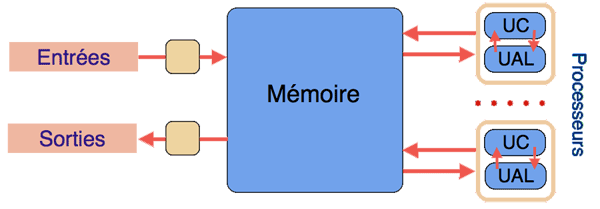
\includegraphics{../img/modele-actuel.png}
	\end{center}
	\caption{Fig. \ref{fig:modelactuel} -- Modèle actuel}
	\label{fig:modelactuel}
\end{figure}

les ordinateurs actuels comportent plusieurs processeurs (on dit aussi
plusieurs \og c\oe urs\fg) intégrés sur une même puce. Cette tendance au
\og parallélisme\fg dans le traitement et la circulation des informations conduit à une augmentation de la puissance de calcul sans augmenter la
fréquence des processeurs individuels.

    \hypertarget{architecture-de-harvard}{%
\section{Alternative: architecture de Harvard}\label{architecture-de-harvard}}

Dans le modèle d'architecture de Harvard les instructions et les données
sont situées dans des mémoires différentes et sont véhiculés sur des bus
indépendants. 
\begin{figure}[h]
	\begin{center}
		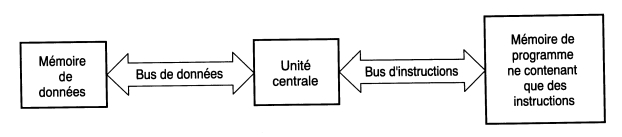
\includegraphics{../img/harvard.001.jpg} 
	\end{center}
	\caption{Fig. \ref{fig:harvard} -- Modèle d'architecture de Harvard}
	\label{fig:harvard}
\end{figure}

La vitesse d'execution
est de fait améliorée car en un seul cycle d'horloge on peut récupérer
les données et le code instruction.\\
\textbf{L'architecture de Harvard se retrouve beaucoup dans les systèmes
embarqués}.


    % Add a bibliography block to the postdoc
\vspace{3cm} 
 Ce(tte) œuvre est mise à disposition selon les termes de la Licence
\href{https://creativecommons.org/licenses/by-nc/4.0/}{Creative Commons Attribution - Pas d'Utilisation Commerciale 4.0
International.}
\begin{center}

\includegraphics{../img/Cc-by-nc_icon.svg.png}
\end{center}      
    
    
    \end{document}
